\documentclass[12pt]{article}
\usepackage[utf8]{inputenc}
\usepackage[figures]{updiplom}
\usepackage{epstopdf,graphicx,dsfont}
\usepackage{listings}%zdrojove kody
\usepackage[usenames,dvipsnames]{color}
\usepackage[hidelinks]{hyperref}

\title{Aplikace Spotting pro OS Android}
\author{Milan Jiříček}
\year{2015}
\docinfo{Milan Jiříček}{Aplikace Spotting pro OS Android}

\annotation{
	Práce se zabývá vývojem aplikace pro systém Android, která umožní uživatelům vyhledání míst pro skateboardery, bikery a bruslaře. Pomocí ní lze vkládat fotky tzv. spotů a skateparků a tato místa vyhledávat a prohlížet podle různých filtrů, jako je vyhledávání podle aktuální polohy, druhu sportu a dalších aspektů. Aplikace dále umožňuje zobrazení vybraných míst na mapě a je zveřejněna pomocí služby Google Play.
}

\thanks{
Děkuji vedoucímu bakalářské práce panu Mgr. Jiřímu Zacpalovi, Ph.D. za konzultace a odborné vedení. Dále bych chtěl poděkovat rodině za jejich podporu při studiích.
}
      
\makeindex

\begin{document}
\maketitle

\newpage

\section{Úvod}
Cílem mé bakalářské práce je mobilní aplikace pro platformu Android, která umožní uživatelům vyhledání míst pro skateboardery, bikery a bruslaře. S rostoucím počtem chytrých telefonů, jsou dnes již tyto přístroje dostupné prakticky komukoliv. Díky tomu mohou aplikace vytvořené pro tyto telefony ulehčit každodenní činnosti a život bez nich si už neumíme představit.

V dnešní době patří mezi nejrozšířenější operační systémy pro chytré telefony Android, iOS a Windows Phone.

Jak je již psáno, pro vývoj aplikace byla zvolena platforma operačního systému Android od společnosti Google. Jedním z kritérií pro volbu OS Android je jeho rozšířenost na trhu, kdy za celý rok 2014 se prodala více než miliarda zařízení s tímto operačním systémem. Dalším z důvodů je osobní vlastnictví mobilního zařízení s tímto systémem a několikaletá zkušenost s každodenním užíváním. V neposlední řadě jsou aplikace pro Android vyvíjeny v programovacím jazyce Java, který je mi velice blízký.

Aplikace, která je pojmenována Spotting, bude sloužit pro vyhledání, přidání a prohlížení míst (tzv.spotů). Spoty bude možno zobrazovat jako místa určená zeměpisnými souřadnicemi na mapě. Ke spotům bude možno vkládat jejich fotografie, které budou moci být otagovány. Aplikace bude obsahovat funkce pro vyhledávání a prohlížení spotů  podle různých filtrů, jako je vyhledávání podle aktuální polohy, druhu sportu a dalších aspektů. Podrobnější funkce aplikace jsou popsány v praktické části bakalářské práce.
\newpage

\section{Platforma Android}
Platforma Android je operační systém založený na Linuxovém jádru, která je v první řadě určená pro mobilní zařízení:
\begin{itemize}
\item chytré telefony
\item navigace
\item PDA
\end{itemize}
Ale můžeme se s ním setkat i např. v MP3 přehrávačích a náramkových hodinkách.
Od jádra přejímá funkce zajišťující bezpečnost systému, správu procesů, paměti a síťí a ovladače všech vnitřních senzorů a komponent. Systém je dostupný jako open source a tím se  liší od konkurenčních firem.

Při vývoji pro mobilní zařízení, se programátor potýká např. s menší výkonností a velikostí paměti v porovnání se stolními počítači. V tomto se snaží Android o kompromis a umožňuje psát aplikace v programovacím jazyce Java a používat většinu knihoven, které se používají pro stolní počítače.
\subsection{Krátká historie}
Kalifornská společnost Android Inc. byla založena v roce 2003. Lidé, kteří stáli u jejího zrodu jsou Andy Rubin, Nick Sears, Richard Miner a Chris White.

V roce 2005 byla prodána společnosti Google Inc. a stala se tak jednou z jejich dceřiných společností.\cite{historie}

 V roce 2007 byla vytvořena skupina Open Handset Alliance. Ta byla složena ze společností zabývající se výrobou mobilních zařízení, čipů nebo aplikací. V jejichž čele stojí společnosti jako je např. Google, HTC, Samsung, Motorola a mnoho dalších. V rámci Open Handset Alliance vydala produkt Android, jako open source, který je nezávislý na použitém hardwaru. Díky tomu, že je open source, výrobci telefonů nemusejí platit za licenci pro jeho použití. To se odráží na cennách telefonů a může být díky tomu i v low-end zařízeních\footnote[1]{zařízení v nízké cenové kategorii}. Tím získalo větší počet uživatelů a dominanci na trhu.
 
\newpage
\subsection{Architektura platformy Android}
Architektura platformy Android se skládá z pěti vrstev a je znázorněna na obr. \ref{architektura} Níže popíši jednotlivé vrstvy.
\begin{figure}[ht]
\centerline{\includegraphics[scale=0.65]{images/architektura.png}}
\caption{Architektura Androidu\cite{architektura}} \label{architektura}
\end{figure}

\begin{itemize}
\item[Linuxové jádro] Nejnižší vrstvou architektury je jádro operačního systému, která zajišťuje komunikaci mezi hardwarem a softwarem. Základ tvoří ovladače, které zajišťují již zmiňovanou komunikaci. Dále poskytuje další základní služby jako jsou např.:
\begin{itemize}
\item správa paměti
\item správa procesů
\item správa napájení
\end{itemize}
\item[Knihovny] Nativní knihovny androidu jsou základními funkcemi. Obsahují např. 
\begin{itemize}
\item Open GL knihovnu pro práci s 3D grafikou.
\item Open SGL pro práci s 2D grafikou.
\item SQLite slouží jako relační databáze pro ukládání a práci s daty.
\item Knihovna médií pro práci s mediálními soubory. Obsahuje kodeky pro různé formáty audia a videa. Například formáty AAC, MPEG4, JPG, PNG.
\item FreeType vektorové a bitmapové vykreslování písma.
\end{itemize}
Tyto funkce jsou poskytnuty vývojářům za pomocí Android Application Framework.
\item[Běhové prostředí Android] Vrstva slouží pro běh aplikací, které jsou psány v programovacím jazyce Java. Ty jsou poté přeloženy do Java byte kódu a následně do mezikódu za pomocí Dalvik kompilátoru. Výsledný byte kód je spuštěný na virtuálním stroji Dalvik. Je navržený tak, že každá aplikace je samotný proces s vlastní instancí virtuálního stroje. Jedním z důvodů, proč nebyl zvolený virtuální stroj (JVM), jsou licenční podmínky. Dalším z důvodů pro zavedení Dalvik byla optimalizace virtuálního stroje pro potřeby mobilních zařízení. Je zřejmé, že hlavní roli hrála úspora energie a především výkon.
Obsahem této vrstvy jsou i knihovny programovacího jazyka Java, ale také knihovny pro zařízení se systémem Android.
\item[Aplikační rámec] Umožňuje přístup k různým službám, které vývojáři mohou používat ve svých aplikacích např.
\begin{itemize}
\item tvorba uživatelského rozhraní.
\item používat hardware zařízení.
\item spouštět jiné aplikace na pozadí.
\end{itemize}
\item[Aplikační vrstva] Je nejvyšší vrstva, v které jsou spuštěny samotné aplikace.
\end{itemize}
\subsection{Volba úrovně API}
Za dobu co je systém Android na trhu, vzniklo několik verzí právě tohoto OS. Zavedl se standart pro psaní programů pro konkrétní verzi systému tzv. úroveň API\footnote[2]{Reprezentuje celočíselnou hodnotu, která jednoznačně identifikuje verzi revize programového vybavení, který je poskytován prostřednictvím dané verze OS. Její hlavní roli je zajištění kompatibility mezi aplikacemi a přístroji, do kterých mají být nainstalovány.}. Proto je před vývojem aplikace velmi důležitá volba cílové verze systému android resp. volba úrovňe API. Může zde dojít k problému, kdy zvolíme příliš novou verzi. Tím můžeme přijít o potenciální zákazníky, kteří mohou naši aplikaci využívat.

Google zveřejňuje statistiky zastoupení jednotlivých verzí OS Android, které přistupují do služby Google Play\footnote[3]{Služba pro stahování hudby, filmů, knih, aplikací a her pro platformu Android, kterou oficiálně provozuje společnost Google.} (viz. obr. \ref{api}).
Na základě těchto údajů se vývojář může rozhodnout, kterou úroveň API zvolí. Pro svoji aplikaci jsem zvolil úroveň API 15 a vyšší. Jedním z důvodů je, že funkce obsažené v knihovnách jsou dostatečné pro můj program a také bude fungovat na více než 90\% zařízeních.
\begin{figure}[ht]
\centerline{\includegraphics[scale=0.65]{images/version.png}}
\caption{Údaje verzí Android přistupující do služby Google Play během sedmi dní k 2. 3. 2015\cite{volba}} \label{api}
\end{figure}
\subsection{Přehled již existujících řešení}
Před výběrem bakalářské práce bylo nutné zjistit, jestli že
neexistují podobné aplikace. Vybrané aplikace byly staženy z Google Play a poté nainstalovány a zkoušeny na mobilním telefonu HTC Evo 3D s verzí OS Android 4.0.3.
\begin{itemize}
\item[Instagram] Jako první zmiňuji právě Instagram a to z důvodu, že má klientská aplikace využije filosofie designu v současné době této populární aplikace. Ta umožňuje svým uživatelům sdílení fotografií. Formát fotografie je odlišný a pořízené snímky jsou ve čtvercovém formátu. Budu využívat i podobné menu, které se  skládá z pěti tlačítek v dolní části obrazovky (viz. obr. \ref{insta}). Dané aplikace se budou od sebe odlišovat převažně ve funkčnosti.

\item[SkateSpots] Je tvořena dvěma částmi menu a pracovní plochou. Hlavní menu je koncipováno formou pěti ikonek ve spodní části displeje. První zleva je hlavní kanál, kde vidíme fotografie posledně nahraných spotů. Hned vedle vpravo se nachází tlačítko, které zobrazí mapu s vyznačenými spoty, dále pro přidání spotu, kde po spuštění mi aplikace přestala pracovat na mobilním telefonu HTC Evo 3D, ale na jiným zařízení fungovalo bez problému. Poté se nachází seznam oblíbených a poslední zobrazí námi nahrané spoty. Z GUI\footnote[4]{Grafické uživatelské rozhraní.} nemám téměř co vytknout. V dané aplikaci mi převážně chybí rozsáhlejší vyhledávání míst podle důležitých aspektů např. do určité vzdálenosti, druhu místa a sportu, daného povrchu, obtížnosti atd. a poté zobrazení vyhledaných spotů, které si bude uživatel moct projít a vybrat si dle sebe.

\item[Tambalea Skate Spots] Po prvním spuštění se zobrazí mapa s vyznačenými spoty, nad ní je menu tzv. Tab bar skládající se ze 4 záložek. V dolní části se nachází tři tlačítka, které jsou nevkusně zvolené obrázky ložiska a skatebordu s popiskem. Za další záložkou se mapa nahradila seznamem spotů, které jsou řazeny pod sebou. Jeden řádek je rozvržen tak, že na levé straně je ikonka označující typ a vedle ní doplňující informace. Vyhledání je zde velice obtížné. Chybí zde obrázek spotu, který u vyhledání hraje jednu z nejvýznamnějších rolí. V dolní části obrazovky se nachází tlačítka pro filtrování seznamu spotů, která jsou opět nevkusně zvolena jako obrázky skateboardů. V další záložce pojmenovanné \uv{MY SPOTS}, by uživatel očekával pouze sebou nahrané, ale nachází se zde i tlačítko pro přidání, které by se hodilo spíše do horního menu. Při přidávání se musíme proklikat mapou pro získání polohy a až poté můžeme pokračovat. Zde mi chybí využití GPS modulu, který je integrovaný ve většině mobilních zařízení. V poslední záložce nastavení se můžeme odhlásit. Po znovu spuštění aplikace se musíme znovu přihlásit, což je velmi otravné.
\end{itemize}
\begin{figure}[ht]
\centerline{\includegraphics[scale=0.18]{images/instagram.png}}
\caption{Úvodní obrazovka aplikace Instagram.} \label{insta}
\end{figure}
\newpage
Analýza aplikací na trhu poukázala na některé nedostatky. K hlavním nedostatkům patří vzhled uživatelského rozhraní, který má rozhodující význam při výběru aplikace uživatele a následným používáním. Dále byly vynechány některé funkce, které by aplikace tohoto typu měla mít. Testování přineslo mnohá ponaučení při vývoji aplikace.

\newpage
\section{Potřebné nástroje při vývoji aplikace}
Vývoj pro platformu Android může být různý. Nejčastěji se používá jazyk Java společně s XML a balíčkem vývojových nástrojů tzv. SDK. Lze využít i další možnost jako je Android NDK, což je balík pro vývoj v jazyce C/C++. My se budeme zabývat vývojem právě v jazyce Java, protože použití NDK, se má používat pouze v případě, pokud to není nezbytně nutné pro fungování aplikace.
\subsection{Java Development Kit}
Java Development Kit (dále JDK) od firmy Oracle, je nezbytný pro vývoj v jazyce Java. Tvoří soubor základních knihoven a nástrojů. Základní součástí je Java Runtime Environment (dále JRE), který slouží pro spouštění aplikací i vývojových nástrojů a obsahuje virtuální stroj a sadu základních knihoven pro vývoj. Nástroje jsou k dispozici pro operační systémy  Linux, Mac OS X, Solaris a Windows.

Některé nástroje obsažené v JDK:
\begin{itemize}
\item java - Spouštěč přeloženého Java byte kódu.
\item javac - Překladač, umožňuje převod  java souboru do Java byte kódu.
\item jdb - Debugger pro ladění programů.
\item javadoc - Generátor dokumentace ze zdrojových kódů.
\item jar - Správce archivů JAR.
\end{itemize}
\subsection{Software Development Kit}
Software Development Kit (dále SDK), je balíček nástrojů pro vývoj aplikací pro platformu Android. Nástroje jsou k dispozici pro operační systémy  Linux, Mac OS X a Windows. Dále si ukážeme nejpoužívanější nástroje.
\newpage
\subsubsection{SDK manager}
Nástroj, který slouží ke správě vašeho SDK balíčku. Poskytuje informace o již nainstalovaných nástrojích a zároveň nám hlídá, aby byly aktuální.
\begin{figure}[ht]
\centerline{\includegraphics[scale=0.5]{images/sdkManager.png}}
\caption{SDK manager ukazující informace o nástrojích.} \label{manager}
\end{figure}
\subsubsection{AVD}
Nedílnou součástí při implementování je ladění, ke kterému je potřeba, aby aplikace byla spuštěna na nějakém zařízení. K tomu nám může sloužit zařízení, které je připojené přes USB\footnote[5]{Univerzální sériová sběrnice. Port pro připojení periferií, přenosných datových úložišť a dalších zařízení.} a je potřeba přepnout do vývojářského módu, nebo můžeme využít emulátoru, který se nazývá Android Virtual Device (dále AVD). Je tedy možné spustit aplikaci a nasimulovat chování téměř všech zařízení s OS Android.

K jeho vytvoření a nastavení konfigurace hardwaru a softwaru slouží AVD manager. Hardwarovou konfiguraci lze měnit dle požadavků pro náš vývoj. Můžeme si nastavit různé parametry. Mezi nejdůležitější patří rozlišení obrazovky, velikost paměti, zda bude mít fotoaparát a další. Z hlediska softwaru se nastavuje úroveň API.

Při vývoji pro Android se bez emulátorů neobejdeme a to z důvodu, že je mnoho zařízení s různými typy obrazovek právě pro tutu platformu. Na obrázku \ref{avd}, můžeme vidět, jak se vytváří nové AVD.
\newpage
\begin{figure}[ht]
\centerline{\includegraphics[scale=0.4]{images/AVD.png}}
\caption{Tvorba AVD.} \label{avd}
\end{figure}

\subsubsection{Dalvik Debug Monitor Server}
Dalvik Debug Monitor Server (dále DDMS) je nástroj, který slouží k ladění spuštěné aplikace, buď na emulátoru nebo fyzickém zařízení. DDMS obsahuje např. modul LogCat, který nám umožňuje sledovat veškeré procesy, které probíhají na zařízení v reálném čase. Také můžeme za pomocí DDMS nasimulovat některé situace, které by při běhu aplikace mohli nastat:
\begin{itemize}
\item příchozí textovou zprávu.
\item příchozí hovor.
\item odeslání informací na zařízení o poloze.
\item a další.
\end{itemize}
\subsubsection{Draw 9-patch}
Je editor pomocí kterého je možné vytvářet bitmapové obrázky, u kterých si lze nastavit body, které se budou při změně velikosti roztahovat. Využívá se např. při vytváření tlačítek, kdy lze jedno tlačítko použít s různými rozměry bez deformací.
\subsection{Vývojové prostředí}
Dalším krokem před vývojem je výběr vývojového prostředí (dále IDE). Tento krok je velice důležitý, protože kvalitní IDE nám může usnadnit práci při vývoji a zvýšit naši produktivitu.
\subsubsection{Eclipse}
Jako první zmiňuji Eclipse IDE, které se používá zejména pro programovací jazyk Java. Zmiňuji ho právě proto, že bylo po dlouhou dobu jako jediné podporováno společností Google pro vývoj aplikací pro platformu Android.

Pro vývoj pro Android v Eclipse se musí doinstalovat plugin Android Development Tools (dále ADT). Je to plugin, který poskytuje sadu nástrojů, které jsou integrovány s IDE. To nabízí přístup k mnoha funkcím. Dále poskytuje GUI přístup k mnoha z SDK nástrojů příkazového řádku, stejně jako nástroj pro návrh uživatelského rozhraní pro rapid prototyping, projektování a budování uživatelského rozhraní vaší aplikace. Toto IDE má jedinou výhodu vzhledem k Android Studiu a tou je podpora NDK. \cite{eclipse}
\subsubsection{NetBeans}
NetBeans IDE se také používá zejména pro programovací jazyk Java, ve kterém je i naprogramován a umožňuje programování i v jiných jazycích jako PHP, C++ a dalších.

Pro vývoj pro NetBeans se také musí doinstalovat plugin NBAndroid\footnote[6]{Open source software distribuovaný pod Apache License 2.0.}. Tento plugin je neoficiální a není podporován společností Google. Na obrázku \ref{netbeans}, můžete vidět Netbeans IDE se spuštěným AVD a na levo od něj můžete vidět LogCat.
\begin{figure}[ht]
\centerline{\includegraphics[scale=0.35]{images/netbeans.png}}
\caption{NetBeans IDE.} \label{netbeans}
\end{figure}
\newpage
\subsubsection{Android Studio}
Jako poslední zmiňuji Android Studio IDE, které je od prosince roku 2014 oficiálně podporováno společností Google. Jeho předchůdcem byl již zmiňovaný Eclipse v kombinaci s pluginem ADT	, jehož vývoj byl ukončen. Toto prostředí je založené na IntelliJ IDEA\footnote[7]{IDE pro programování v jazycích Java, Groovy a dalších.}.

Instalace probíhá narozdíl od Eclipse a NetBeans velice jednoduše. Stačí si stáhnout a nainstalovat instalační balík. K instalaci je potřeba Java od společnosti Oracle. Jak jste si určitě všimli, nejsou potřeba žádné pluginy. \cite{studio}

\subsubsection{Výběr IDE}
Výběr IDE byl velice složitý. Hlavním z důvodů mého výběru bylo, že v dané době Android Studio bylo ještě ve vývoji a oficiálně byl podporován pouze Eclipse. Takže mně zůstal výběr mezi NetBeans a Eclipse. Po dlouhém rozmýšlení, jsem si vybral NetBeans a to z důvodu, že s ním mám dobré a velké zkušenosti narozdíl od Eclipse. Po dobu vývoje jsem se nesetkal s žádným větším problémem s IDE.

Nyní kdybych si měl zvolit, bylo by to jednoznačně Android Studio a to z důvodu, že se obvykle vyžadují zkušenosti pro přijetí do práce s tímto IDE a práce s ním má jisté výhody:
\begin{itemize}
\item oficiální podpora.
\item rychlost.
\item menší spotřeba paměti.
\end{itemize}
\newpage
\section{Základy vývoje Android aplikací}
Aplikace pro Android sestávájí z několika komponent activities (aktivity), services (služby), content providers (poskytovatelé obsahu) a broadcast recievers (přijímače). Komponenty jsou deklarovány v souboru AndroidManifest.xml, který specifikuje celou aplikaci. Na základě tohoto souboru systém ví, co lze jak volat a jak může komponenta spolupracovat s okolím. V této sekci si popíšeme k čemu slouží a jejich životní cyklus, který určuje jak komponenta vzniká a zaníka. Informace jsou převzaty ze zdroje \cite{slozeni}.
\subsection{Aktivity}
V aplikaci reprezentují prezentační vrstvu. Káždá aktivita obvykle odpovídá jedné obrazovce aplikace. Slouží tedy jako hlavní prostředek pro interakci s uživatelem, i když je možné, aby neměly uživatelské rozhraní, ale v této práci se s tím nesetkáme. UI lze definovat dvěma způsoby:
\begin{enumerate}
\item v XML souboru.
\item za běhu programově.
\end{enumerate}
Tyto dva způsoby lze i kombinovat. Obvykle se definuje výchozí vzhled pomocí XML souboru a potom při uživatelově interakci se může tento vzhled za běhu měnit.

Aplikace většinou obsahují více aktivit, které jsou mezi sebou vázány a jedna z nich je určená jako hlavní. Ta se zobrazí ihned po spuštění aplikace. Aktivita může za pomocí záměrů mezi jednotlivými aktivitami přepínat a předávat data. Vždy, když začne nová aktivita, předchozí aktivita se zastaví a uloží do zásobníku, ale je možné se k ní vrátit za pomocí tlačítka zpět.
\subsubsection{Životní cyklus aktivit}
OS Android se nechází převážne na mobilních zařízeních, které trpí nedostatkem operační paměti. Je zřejmé, že některé aktivity jsou důležité a některé méně. Proto v důsledku nedostatku operační paměti je možné násilné ukončení aktivity z důvodu, kdy systém potřebuje uvolnit paměť jiné aktivitě. V této sekci si popíšeme životní cyklus aktivit tzn. popis stavů, ve kterých se může nacházet nebo událostí od jejího vzniku až po její ukončení.

Každá aktivita prochází vlastním životním cyklem a nachází se v jednom z následujích čtyř stavů:
\begin{itemize}
\item aktivní - Aktivita je spuštěna a běží v popředí.
\item pozastavená - Aktivita je spuštěna, běží a je viditelná, ale uživatel s ní nemůže interagovat. To bývá způsobeno částečným překrytím aktivity jinou, která nezabírá celou obrazovku nebo je z části průhledná. Tato situace většinou nastane při zobrazení dialogového okna.
\item zastavená - Aktivita je spuštěna, běží, ale není viditelná, je překryta jinými aktivitami. Nyní může být aktivita ukončena, pokud je potřeba uvolnit paměť.
\item mrtvá - Aktivita nebyla spuštěna, nebo byla ukončena  násilně z důvodu nedostatku duspné paměti, nebo jí ukončil uživatel. Jestliže má být aktivita znovu spuštěna do popředí, je potřeba jí znovu vytvořit.
\end{itemize}
\subsubsection{Callback metody}
Systém při přecházení mezi jednotlivými stavy volá callback metody. Životní cyklus aktivity a přecházení mezi stavy je znázorněno na obr. \ref{lifecycle}.

\begin{itemize}
\item metoda onCreate() se volá při prvním spuštění aktivity. V této metodě se inicializuje UI a provádí se zde veškeré operace, které je potřeba provést pouze jednou a nejsou závislé na dalším způsobu použití aktivity. Metoda se také volá v případě, pokud běžela a změnily se jí prostředky, které aktivita využívá ke své činnosti a je potřeba ji znovu vytvořit. K tomuto dochází např. při změně orientace obrazovky, kdy je nutné znovu vytvořit UI.
\item metoda onDestroy() je volána při ukončování aktivity. Tato metoda se hodí pro uvolnění prostředků, které jsme získali při vytváření aktivity. Je volána vždy, když je aktivita ukončena funkcí finish(), ale pokud je ukončena násilně z důvodu nedostaku dostupné paměti nemusí k volání metody dojít.
\item metoda onRestart() se volá tehdy, když byla aktivita zastavena a má se znovu spustit.
\item metoda onStart() se volá před tím, než se stane aktivita viditelnou.
\item metoda onResume() se volá těsně před přesunem aktivity do popředí. Zde je možné si změnit UI na základě nějaké události, která nastala.
\item naopak metoda onPause() je volána, pokud se do popředí dostane jiná aktivita. Zde je výhodné zrušit vše, co jste provedli v metodě onResume() např. ukončení všech procesů mimo hlavní vlákno, uvolnění všech prostředků(např. fotoaparát), které si aktivita vyžádala atd.
\item metoda onStop() se volá tehdy, když aktivita není viditelná.
\end{itemize}
\newpage
\begin{figure}[ht]
\centerline{\includegraphics[scale=0.68]{images/lifecycle.png}}
\caption{Životní cyklus aktivit.} \label{lifecycle}
\end{figure}
\subsection{Intenty}
Intenty jsou základními komunikačními prvky mezi jednotlivými komponentami aplikace. Je to tedy objekt třídy Intent, který slouží pro spuštění aktivity nebo služby a dokáže přenášete jednoduchá data mezi těmito komponentami. Rozdělujeme je na explicitní a implicitní:
\begin{itemize}
\item explicitní - Používají se ke spuštění jedné konkrétní aktivity. Systém přesně ví, jak reagovat.
\definecolor{lightGrey}{RGB}{250,250,250}

\begin{lstlisting}[language=Java,
title=Ukázka explicitního intentu.,
basicstyle=\ttfamily\small\color{black},
commentstyle=\itshape,
keywordstyle=\color{Blue},
showstringspaces=false,
frame=lines,
backgroundcolor=\color{lightGrey}
]
Intent i = new Intent(context, CameraActivity.class);
\end{lstlisting}
\item implicitní - Používají se v případě, kdy je jasné co má být provedeno, ale není definované jak danou činnost provést, to necháme na systému.
\begin{lstlisting}[language=Java,
title=Ukázka implicitního intentu.,
basicstyle=\ttfamily\small\color{black},
commentstyle=\itshape,
keywordstyle=\color{Blue},
showstringspaces=false,
frame=lines,
backgroundcolor=\color{lightGrey}
]
Uri uri = Uri.parse("http://www.spotting.com");
Intent i = new Intent(Intent.ACTION_VIEW, uri);
startActivity(i);
\end{lstlisting}
Na příkladu můžete vidět otevření webové stránky z aktivity pomocí nějakého internetového prohlížeče.
\end{itemize}
\subsection{Poskytovatelé obsahu}
Jak jsem zmiňoval výše, lze přes intenty posílat a přijímat menší množství dat, které se ale nehodí pro větší objemy dat. Z tohoto důvodu jsou v systému poskytovatelé obsahu, kteří jsou určení ke sdílení dat mezi jednotlivými aplikacemi v celém systému. Systém je dodáván s poskytovateli obsahu pro některé zakladní typy dat a řadu z nich najdeme v balíčku Android.provider. Jestliže chceme sdílet některá data, je to možné dvojím způsobem:
\begin{enumerate}
\item a to vytvořením vlastního poskytovatele obsahu za pomocí třídy contentProvider\footnote[8]{Komponenta spravující sdílená aplikační data.}.
\item nebo využitím stávajícího poskytovatele obsahu, kdy musí poskytovat stejný typ dat a také musíte mít povolený přístup pro zápis.
\end{enumerate}
\subsection{Služby}
Aktivity a poskytovatelé obsahu jsou entity s krátkou životností, které lze kdykoliv vypnout. Proto existují služby, které jsou navrženy tak, aby mohli provádět dlouhotrvající operace na pozadí. Služby neposkytují GUI a nejsou proto vázány na grafické rozhraní aplikace. Např. lze tedy přehrávat hudbu, i když aktivita, při které bylo spuštěno přehrávání, už byla ukončena.
\subsection{Přijímače}
Komponenta odvozená od třídy android.app.BroadcastReceiver slouží k naslouchání oznámení. Poté umožňuje reagovat aplikaci na nějakou událost, která nemusela vzniknout v rámci aplikace, ale mohla vzniknout systémem nebo jinou aplikací. Příkladem může být oznámení o příchodu sms zprávy.

\section{Návrh aplikace}
%V této části se budu zabývat programátorskými aspekty práce. Zaměřuje se na architekturu aplikace, dále popisuje knihovny použité při tvorbě aplikace.
V této části se budu zabývat návrhem aplikace, která mi poskytne následné informace k samotné implementaci. Zaměřuji se na popis diagramu případu užití, návrhu architektury a popisu použitých knihoven.
\subsection{Diagram případů užití}
Diagram případu užití znázorněn na obr. \ref{diagram} popisuje funkční požadavky na
\begin{figure}[ht]
\centerline{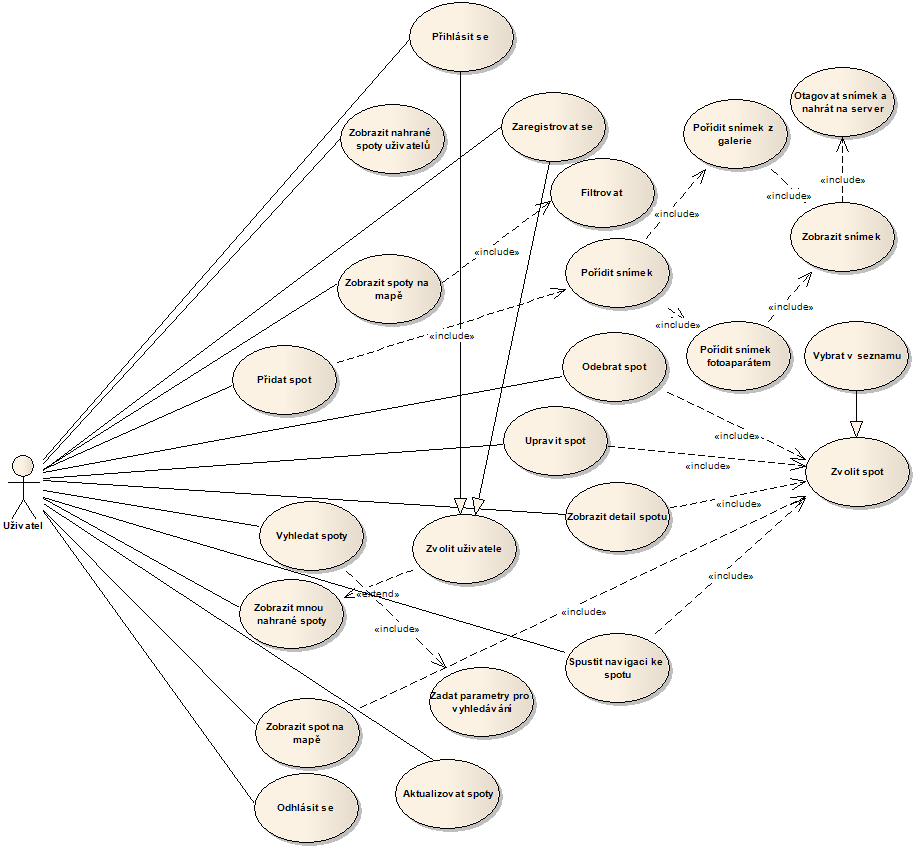
\includegraphics[scale=0.5]{images/spotting-diagram.png}}
\caption{Diagram případů užití aplikace.} \label{diagram}
\end{figure}
systém. Zobrazuje jednotlivé případy užití, které nám znázorňují interakce mezi uživatelem  aplikace a aplikací samotnou.
%http://dspace.upce.cz/bitstream/10195/53642/2/ZamazalJ_NavrhAplikace_JP_2013.pdf
\subsection{Architektura aplikace}
Součástí systému je serverová část a klientská android aplikace komunikující s tímto serverem. Komunikace mezi android klientem a serverem je skrz REST\footnote[9]{Representational State Transfer - architektura webových aplikací, která nám umožňuje přistupovat k datům.} služby. Jako datové úložiště je zvoleno MySQL.

Využívám tedy třívrstvé architektury, kdy je aplikace rozdělena na to co uživatel vidí a na to, co se odehrává na pozadí na straně serveru.

Vrstvy architektury:
\begin{itemize}
\item Prezentační vrstva - Klientská mobilní aplikace pro platformu Android.
\item Aplikační vrstva - Prostředník mezi prezentační a datovou vrstvou. Je tvořena PHP skripty společně s SQL příkazy, které běží na webovém serveru. Zvolil jsem free hostingový server Endora.cz, který splňoval nejlépe mé požadavky např. bezplatnou registraci domény III. řádu, bezplatný hosting a podporu MySQL databází.
\item Datová vrstva - Její úlohou je ukládání dat do perzistentního uložiště. V mém systému, jak jsem již zmiňoval byla zvolena relační databáze MySQL.
\end{itemize}
Výhodou zvolené architektury je rozdělení výkonu mezi zařízení uživatele a serveru. Díky tomuto může běžet i v low-end zařízeních.
\subsection{Použité knihovny}
Při vývoji byla použita i řada externích knihoven, které si v této kapitole rozebereme.
\subsubsection{Volley}
Je knihovna vyvíjená společností Google, která slouží pro snadnější a hlavně rychlejší používání síťových požadavků. Mezi její výhody patří automatické plánování síťových požadavků, umožnění více souběžných připojení k síti, poskytnutí paměťového cachování a také umožňuje zrušit pouze jednu nebo všechny žádosti.

Její nevýhodou je, že nedokáže stahovat větší soubory, z důvodu, že udržuje všechny odpovědi v paměti.\cite{volley}
\subsubsection{Google Play Services}
Google Play Services je soubor služeb, jejichž hlavním účelem je ulehčení práce vývojářům. V této aplikaci využívám služby pro získání polohy od nejlepšího poskytovatele a přístup k Google Maps.

Jestliže knihovna Google Play Services není nainstalována na zařízení, tak služby na daném zařízení nebudou fungovat.\cite{services}


Další použité knihovny (httpclient-4.3.6, httpcore-4.3.3, httpmime-4.3.6) viz. kapitola \ref{knihovny}
\section{Impplementace}
\subsection{Odeslání souboru}
\label{knihovny}
%http://is.muni.cz/th/374489/fi_b/BakalarskaPraca.pdf
\newpage
\begin{thebibliography}{1} %při použití psát \cite{vobecky} apod
\bibitem{historie} Google Buys Android for Its Mobile Arsenal. In: \emph{Businessweek - Business News, Stock market \& Financial Advice} [online]. 16. 8. 2005 [cit. 2. 4. 2015]. Dostupné
z: \url{http://www.bloomberg.com/bw/stories/2005-08-16/google-buys-android-for-its-mobile-arsenal}
\bibitem{architektura} Android (operating system). In: \emph{Wikipedia, the free encyclopedia} [online]. 29. 6. 2012 [cit. 2. 4. 2015]. Dostupné z: \url{http://en.wikipedia.org/wiki/File:Android-System-Architecture.svg}

\bibitem{volba} Google Inc. Android Platform Version. In: \emph{Android Developers}
[Online]. 2. 3. 2015 [Citace: 3. 4. 2015]. Dostupné z: \url{http://developer.android.com/about/dashboards/index.html#Platform}

\bibitem{studio} Google Inc. Android Studio In: \emph{Android Developers}
[Online]. 2015 [Citace: 13. 5. 2015]. Dostupné z: \url{http://developer.android.com/tools/studio/index.html}

\bibitem{eclipse} Google Inc. Eclipse with ADT In: \emph{Android Developers}
[Online]. 2015 [Citace: 13. 5. 2015]. Dostupné z: \url{http://developer.android.com/tools/help/adt.html}

\bibitem{slozeni} GRANT Allen \emph{Android 4}
	Brno: Computer Press, 2013.
		[Citace: 13. 5. 2015]

\bibitem{volley} Google Inc. Volley library In: \emph{Android Developers}
[Online]. 2015 [Citace: 14. 7. 2015]. Dostupné z:
\url{https://developer.android.com/training/volley/index.html}

\bibitem{services} Google Inc. Google Play Services In: \emph{Android Developers}
[Online]. 2015 [Citace: 14. 7. 2015]. Dostupné z:
\url{https://developers.google.com/android/guides/overview#the_google_play_services_client_library}
\end{thebibliography}
\end{document}

\definecolor{lightGrey}{RGB}{250,250,250}

\begin{lstlisting}[language=Java,
title=Deklarace,
basicstyle=\ttfamily\small\color{black},
commentstyle=\itshape,
keywordstyle=\color{Blue},
showstringspaces=false,
frame=lines,
backgroundcolor=\color{lightGrey},
numbers=left ,
numberstyle=\small ,
stepnumber=5,
framexleftmargin=10mm,
xleftmargin=10mm,
breakindent=20em,
breakatwhitespace=true ,
breaklines=true]
	int i = 100;
	i++;
	std::cout << i << std::endl;
\end{lstlisting}